\section{Resultados}
Nesta seção, será debatido acerca dos resultados obtidos por meio dos dois testes realizados. O primeiro visou analisar o tempo médio de cada algoritmo, bem como a sua variância. 
No segundo teste, por outro lado, buscou-se avaliar o comportamento dos algoritmos bolha e inserção quando submetidos a vetores com diferentes taxas de ordenação, sendo estas 1\%, 3\%, 5\%, 10\% e, por fim, 50\%. 


\subsection{Variação na quantidade de elementos}
Como comentado, os resultados comprovam o comportamento quadrático do bolha, seleção e inserção. 
Entretanto, é preciso ressaltar que, se existisse uma variação significativa nos números da lista a ser ordenada, o algoritmo de contagem apresentaria um tempo para ordenar maior, podendo ultrapassar o bolha, por exemplo.

\begin{figure}[h]
    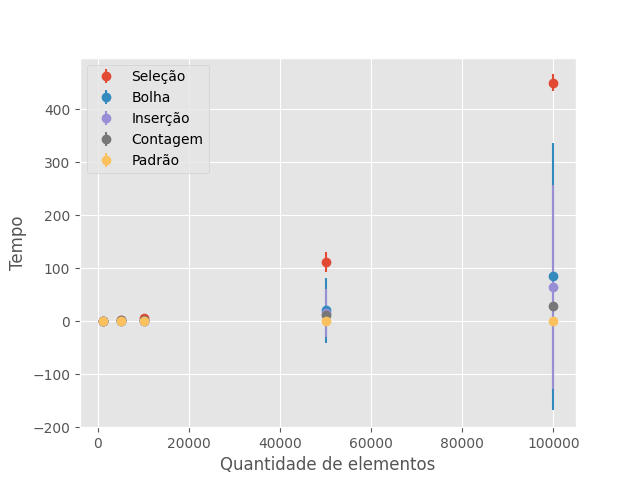
\includegraphics[width=8cm]{sizes.png}
    \caption{Gráfico elucidando o comportamento de cada algoritmo em tópico. No eixo x, há a quantidade de elementos; no eixo y, o tempo médio gasto em segundos}
    \end{figure}

    \begin{table}[h]
        % \centering
        \begin{tabular}{llllll}
            \textbf{Tamanho da lista} & \textbf{Seleção} & \textbf{Inserção} & \textbf{Bolha} & \textbf{Contagem} \\
            1000 & 0.04597 & 0.05796 & 0.06942 & 0.24648 \\
            5000 & 0.98705 & 1.42168 & 1.84406 & 1.21472 \\
            10000 & 3.88312 & 5.79583 & 7.49110 & 2.90298 \\
            50000 & 97.74410 & 148.20082 & 194.80364 & 14.39026 \\
            100000 & 389.11648 & 596.82038 & 791.78906 & 28.75249 \\
        \end{tabular}
        \caption{Tempos de execução dos algoritmos de ordenação (em segundos) para diferentes tamanhos de lista}
        \label{tab:tempos_algoritmos}
    \end{table}

O bolha, apesar de variar dependendo da taxa de ordenação, possui o maior tempo necessário para ordenar. Em seguida, o algoritmo de inserção detém o segundo maior período para organizar a sequência, e isso se dá pelo fato de que o inserção possui uma complexidade quadrática independente da posição inicial dos elementos. 

O algoritmo de seleção, como esperado, contém o melhor tempo de resposta dentre os algoritmos de comparação, tendo em vista que, além de ser mais eficiente em listas com alguns elementos ordenados, realiza menos permutações que o bolha. 

Por último, o contagem apresentou o melhor desempenho dos implementados. Contudo, é necessário destacar que o contagem obteve este performance devido à faixa de números aleatórios escolhida (de 0 a 9999), pois, como analisado, o algoritmo em questão varia com os números recebidos.

Assim, percebe-se que, para listas com muitos elementos, o algoritmo contagem é o mais eficiente entre os implementados, enquanto o bolha apresentou o resultado menos satisfatório para o teste.


\subsection{Ordenação prévia}
\begin{figure}[h]
    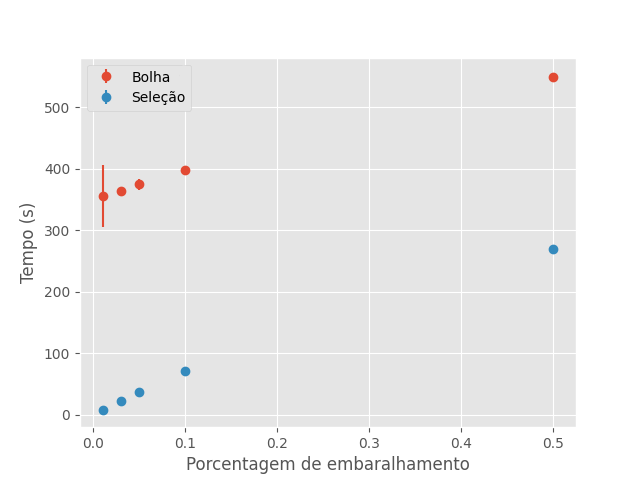
\includegraphics[width=8cm]{percentages.png}
    \caption{Gráfico ilustrando o tempo médio 'gasto' dos algoritmos bolha e inserção em relação à taxa de ordenação inicial dos vetores.}
\end{figure}
\begin{table}[h]
    \begin{tabular}{lcc}
        \textbf{Tamanho da lista} & \textbf{Bolha} & \textbf{Contagem} \\
        1000 & 3.4037e-08 & 1.0778e-05 \\
        5000 & 1.3713e-04 & 5.0052e-05 \\
        10000 & 1.5767e-03 & 1.3368e-03 \\
        50000 & 4.9661 & 0.0697 \\
        100000 & 15.7575 & 1.2251 \\
    \end{tabular}
    \caption{Desvios padrão dos tempos de execução dos algoritmos de ordenação (em segundos) para diferentes tamanhos de lista}
    \label{tab:desvios_algoritmos}
\end{table}

Inicialmente, quando ambos os algoritmos são submetidos a uma lista já ordenada, o tempo de execução do algoritmo de seleção é quase imediato; o bolha, por outro lado, possui uma duração considerável para verificar que a lista já está ordenada. Adicionalmente, ao aumentar a permutação dos elementos, o bolha mantém a sua alta duração, principalmente devido à quantidade de comutações realizadas por este.

Por outro lado, o algoritmo de seleção apresentou um crescimento maior quando intensificada a desordenação da lista, uma vez que a quantidade de comutações realizadas pelo algoritmo tende a se aproximar a do bubble, ou seja, quanto mais ordenada a lista, mais eficiente o seleção é em comparação ao segundo.

Portanto, o algoritmo de seleção é mais eficiente do que o bolha, ainda quando submetido a sequências com diferentes taxas de ordenação. Contudo, o seleção possui uma taxa de crescimento ligeiramente maior do que o bolha quando aumentada a porcentagem de embaralhamento.
